\documentclass[12pt,a4paper]{article} %437
\usepackage{indentfirst}
\usepackage{amsmath}
\usepackage{enumerate}
\usepackage{amssymb}
\usepackage{graphicx}
\usepackage{color}
\makeatletter
\makeatother
\usepackage[brazilian]{babel}
\usepackage[utf8]{inputenc}
\usepackage[T1]{fontenc}
\usepackage{pdflscape}
\usepackage{bm}
\usepackage{float}
%\usepackage[dvips]{graphicx, color}
\usepackage{subfigure}
\usepackage[skins,listings,breakable]{tcolorbox}

\usepackage{color}
\definecolor{lbcolor}{rgb}{0.9,0.9,0.9} 

%TCIDATA{OutputFilter=latex2.dll}
%TCIDATA{LastRevised=Friday, February 01, 2008 17:54:39}
%TCIDATA{<META NAME="GraphicsSave" CONTENT="32">}


\setlength\topmargin{-1.5cm} \setlength\oddsidemargin{0.0cm}
\setlength\evensidemargin{0.0cm} \setlength{\textwidth}{16cm}
\setlength{\textheight}{25cm}


\newtheorem{definition}{Definition}
\newtheorem{theorem}{Theorem}
\newtheorem{example}{Example}
\newtheorem{corollary}{Corollary}
\newtheorem{lemma}{Lemma}
\newtheorem{proposition}{Proposition}
\newenvironment{proof}{{\bf Proof:\ \ }}{\qed}
\newcommand{\qed}{\rule{0.5em}{1.5ex}}
\newcommand{\bfg}[1]{\mbox{\boldmath $#1$\unboldmath}}
\newcommand{\dse} {\displaystyle}
\newcommand{\real}{{I\!\!R}}
\newcommand{\zern}{{\bf 0}}
\newcommand{\Cn}{{\bf C}}
\newcommand{\dn}{{\bf d}}
\newcommand{\Dn}{{\bf D}}
\newcommand{\Pn}{{\bf P}}
\newcommand{\xn}{{\bf x}}
\newcommand{\Un}{{\bf U}}
\newcommand{\Kn}{{\bf K}}
\newcommand{\Xn}{{\bf X}}
\newcommand{\Vn}{{\bf V}}
\newcommand{\vn}{{\bf v}}
\newcommand{\bn}{{\bf b}}
\newcommand{\an}{{\bf a}}
\newcommand{\cn}{{\bf c}}
\newcommand{\en}{{\bf e}}
\newcommand{\sn}{{\bf s}}
\newcommand{\Bn}{{\bf B}}
\newcommand{\An}{{\bf A}}
\newcommand{\yn}{{\bf y}}
\newcommand{\Yn}{{\bf Y}}
\newcommand{\Zn}{{\bf Z}}
\newcommand{\zn}{{\bf z}}
\newcommand{\Hn}{{\bf H}}
\newcommand{\Gn}{{\bf G}}
\newcommand{\Mn}{{\bf M}}
\newcommand{\fn}{{\bf f}}
\newcommand{\hn}{{\bf h}}
\newcommand{\In}{{\bf I}}
\newcommand{\Fn}{{\bf F}}
\newcommand{\En}{{\bf E}}
\newcommand{\Jn}{{\bf J}}
\newcommand{\Ln}{{\bf L}}
\newcommand{\mn}{{\bf m}}
\newcommand{\rn}{{\bf r}}
\newcommand{\un}{{\bf u}}
\newcommand{\Rn}{{\bf R}}
\newcommand{\Sn}{{\bf S}}
\newcommand{\Tn}{{\bf T}}
\newcommand{\GLn}{{\bf G \bf L}}
\newcommand{\tn}{{\bf t}}
\newcommand{\alpn}{{\mbox{\boldmath $\alpha$}}}
\newcommand{\epsiln}{{\mbox{\boldmath $\epsilon$}}}
\newcommand{\rhn}{{\mbox{\boldmath $\rho$}}}
\newcommand{\betn}{{\mbox{\boldmath $\beta$}}}
\newcommand{\deltn}{{\mbox{\boldmath $\delta$}}}
\newcommand{\sigmn}{{\mbox{\boldmath $\beta$}}}
\newcommand{\gamn}{{\mbox{\boldmath $\gamma$}}}
\newcommand{\Gamn}{{\mbox{\boldmath $\Gamma$}}}
\newcommand{\lamn}{{\mbox{\boldmath $\lambda$}}}
\newcommand{\Lamn}{{\mbox{\boldmath $\Lambda$}}}
\newcommand{\mun}{{\mbox{\boldmath $\mu$}}}
\newcommand{\etn}{{\mbox{\boldmath $\eta$}}}
\newcommand{\tetn}{{\mbox{\boldmath $\theta$}}}
\newcommand{\Tetn}{{\mbox{\boldmath $\Theta$}}}
\newcommand{\Deltn}{{\mbox{\boldmath $\Delta$}}}
\newcommand{\Phin}{{\mbox{\boldmath $\Phi$}}}
\newcommand{\phin}{{\mbox{\boldmath $\phi$}}}
\newcommand{\Psin}{{\mbox{\boldmath $\Psi$}}}
\newcommand{\psin}{{\mbox{\boldmath $\psi$}}}
\newcommand{\Upin}{{\mbox{\boldmath $\Upsilon$}}}
\newcommand{\upin}{{\mbox{\boldmath $\upsilon$}}}
\newcommand{\Sign}{{\mbox{\boldmath $\Sigma$}}}
\newcommand{\Omegn}{{\mbox{\boldmath $\Omega$}}}
\newcommand{\omegn}{{\mbox{\boldmath $\omega$}}}
\newcommand{\eln}{{\mbox{\boldmath $\ell$}}}
\newcommand{\taun}{{\mbox{\boldmath $\tau$}}}

\hyphenation{ge-ne-ra-ted  hy-per-geo-me-tric  cha-rac-te-ri-ze}


\begin{document}

\begin{center}
\section*{\centerline {A new family of continuous distributions: properties and applications}}
\vspace{0.3in}
{\large Gauss M. Cordeiro$^a$ , Maria do Carmo$^a$ and Pedro Rafael D. Marinho$^b$}\\
%\vspace{0.3in}
%First Version: 27 July 2010\\
%\vspace{0.1in}
%This Version: 27 January 2011\\
\end{center}

\begin{abstract}\noindent
This article introduces generalized beta-generated (GBG) distributions. Sub-models
include all classical beta-generated, Kumaraswamy-generated and exponentiated
distributions. They are maximum entropy distributions under three intuitive
conditions, which show that the classical beta generator skewness parameters
only control tail entropy and an additional shape parameter is needed to add entropy
to the center of the parent distribution. This parameter controls skewness
without necessarily differentiating tail weights. The GBG class also
has tractable properties: we present various expansions for moments,
generating function and quantiles. The model parameters
are estimated by maximum likelihood and the usefulness of the new class
is illustrated by means of some real data sets.
\end{abstract}

\vspace{0.5in}
\noindent {\bf Key Words}: \\ \\
%\noindent {\bf JEL Codes}: C16, G1 \\ \\
\noindent $^{a}$  Department of Statistics, Federal University of Pernambuco, Recife, Brazil.\\
\noindent $^{b}$ Department of Statistics, Federal University of Paraíba, João Pessoa, Brazil.\\
E-mail:\emph{gausscordeiro@de.ufpe.br, maria@de.ufpe.br, pedro.rafael.marinho@gmail.com} \\


\section{Introduction}

There has been an increased interest in developing generalized families of distributions by
introducing additional shape parameters to a baseline cumulative distribution. This mechanism has
proved to be useful to make the generated distributions more flexible especially for studying tail properties
than existing distributions and for improving their goodness-of-fit statistics
to the data under study.

Let $G(x)$ be the cumulative distribution function (CDF) of a
baseline distribution and $g(x)=dG(x)/dx$ be the associated
probability density function (PDF) depending on a parameter vectot $\eta$. We present a generalized family
with two additional shape parameters by transforming the CDF $G(x)$
according to two sequential important gene\-rators. These families are important for modeling data
in several engineering areas. Many special distributions in these families are discussed by Tahir
and Nadarajah (2015).


Marshall and Olkin (1997) pioneered a general method to expand
a distribution G by adding an extra shape parameter.
The CDF of their family (for $\theta>0$) is
\begin{equation}\label{CDF_MO}
F_{\text{MO-G}}(x)=\frac{G(x)}{\theta+(1-\theta)G(x)}=\frac{G(x)}{1-(1-\theta)[1-G(x)]},\quad x \in \mathbb{R}.
\end{equation}

The density function corresponding to (\ref{CDF_MO}) is
\begin{equation}\label{densityMO}
f_{\text{MO-G}}(x)=\frac{\theta g(x)}{[\theta+(1-\theta)G(x)]^{2}},\quad x \in \mathbb{R}.
\end{equation}
For $\theta = 1$, $f_{\text{MO-G}}(x)$ is equal to $g(x)$ and, for different values of
$\theta$, $f_{\text{MO-G}}(x)$ can be more flexible than $g(x)$.
The extra parameter $\theta$ is called ``tilt parameter'', since
the HRF of the MO-G family is shifted below ($\theta> 1$)
or above ($0<\theta<1$) of the baseline HRF. Equation \eqref{densityMO} provides a useful
mechanism to generate new distributions from existing ones. The advantage of this approach
for constructing new distributions lies in its flexibility to model
both monotonic and non-monotonic HRFs even when the baseline HRF may be
monotonic. Tahir and Nadarajah (2015, Table 2) presented thirty distributions belonging to
the $\text{MO-G}$ family. Further, this family is easily generated from the baseline QF by
$Q_{\text{MO-G}}(u)=Q_{G}\left(\theta u \left[\theta u+1-u\right]\right)$ for $u\in(0,1)$.

Marshall and Olkin considered the exponential and Weibull distributions for the baseline G and derived some
structural properties of the generated distributions. The special case that G is an exponential distribution
refers to a two-parameter competitive model to the Weibull and gamma distributions.
A simple interpretation of (\ref{CDF_MO}) can be given as follows. Let $T_1,\ldots,T_N$ be a sequence
of independent and identically distributed (i.i.d.)~random variables with survival function (SF)
$\overline{G}(x)=1-G(x)$, and let $N$ be a positive integer
random variable independent of the $T_i$'s defined by the probability generating function (PGF) of a
geometric distribution with parameter $\theta$, say $\tau(z;\theta)=\theta z\,[1-(1-\theta)z]^{-1}$.
Then, the inverse of $\tau(z;\theta)$ becomes $\tau^{-1}(z;\theta)=\tau(z;\theta^{-1})$. We can verify that
equation \eqref{CDF_MO} comes from $1 - F_{\text{MO-G}}(x)=\tau(\overline{G}(x);\theta)$ for $0<\theta<1$ and
$1-F_{\text{MO-G}}(x)=\tau(\overline{G}(x);\theta^{-1})$ for $\theta>1$. For both cases, $1-F_{\text{MO-G}}(x)$
re\-presents the SF of $\min\{T_1,\ldots,T_N\}$, where $N$ has
PGF $\tau(z;\cdot)$ with probability parameters $\theta$ or $\theta^{-1}$.

Zografos and Balakrishnan (2009) and Risti\'{c} and Balakrishnan (2011)
defined the gamma-G ($\Gamma$-G) family with an extra shape parameter $a>0$ by
the CDF (for $x \in \mathbb{R}$)
\begin{eqnarray}\label{CDF_Ga}
F_{\Gamma\text{-G}}(x)=\gamma_1\left( a, -\log \left[1-G(x)\right]\right)
=\frac{\displaystyle 1}{\displaystyle \Gamma(a)}\,\gamma\left( a, -\log \left[1-G(x)\right]\right),
\end{eqnarray}
where $\gamma(a,z)=\int_0^{z} t^{a-1}\,\rm{e}^{-t}dt$ is the incomplete gamma function and
 $\gamma_1(a,z)= \gamma(a,z)/\Gamma(a)$ is the incomplete gamma function ratio.
The PDF of the $\Gamma$-G family takes the form
\begin{eqnarray}\label{PDF_Ga}
\displaystyle
f_{\Gamma\text{-G}}(x)=\frac{\displaystyle 1}{\displaystyle \Gamma(a)} \left\{ -\log[1-G(x)] \right\}^{a-1}\, g(x),
\quad x \in \mathbb{R}.
\end{eqnarray}
Each new $\Gamma$-G distribution can be determined from a given baseline distribution.
For $a=1$, the G distribution is a basic exemplar of the $\Gamma$-G family.

Zografos and Balakrishnan (2009) and Risti\'{c} and Balakrishnan (2011)
presented a physical motivation for the $\Gamma$-G family: if $X_{L(1)},\ldots, X_{L(n)}$ are lower record values
from a sequence of independent random variables with common PDF $g (\cdot)$, then the PDF of the $n$th lower
record value has the form (\ref{PDF_Ga}). If $Z$ is a gamma random variable with unit scale
parameter and shape parameter $a>0$, then $X=Q_G(1-\rm{e}^{Z})$ has density (\ref{PDF_Ga}). So,
the $\Gamma$-G distribution is easily generated from the gamma distribution and the QF of G.


The rest of the paper is organized as follows. Section \ref{sec:MOGaG} describes the distribution and density
of the new class of distributions called the {\it Marshall and Olkin-Gamma-G} (MO-$\Gamma$-G) family  by combining the above generators.
We also present some special models. The maximum likelihood estimation of the model parameters of the new family is
described in Section \ref{estimation}. In Section \ref{applications}, we provide some empirical applications to illustrate
the potentiality of the proposed family. A variety of theoretical properties are considered in Section \ref{properties}.
Finally, conclusions are noted in Section \ref{conclusions}.


\section{The New Family}\label{sec:MOGaG}

Let $X\sim$MO-$\Gamma$-G denote a random variable having the MO-$\Gamma$-G family with two extra shape parameters $\theta>0$ and $a>0$
and the baseline vector $\eta$. By combining Equations (\ref{CDF_MO}) and (\ref{CDF_Ga}), the CDF of $X$ has the form
\begin{equation}\label{CDF_MO-Gamma-G}
F_{X}(x)=\frac{\gamma_1\left( a, -\log \left[1-G(x)\right]\right)}{\theta+(1-\theta)\gamma_1\left( a, -\log \left[1-G(x)\right]\right)},\quad x \in \mathbb{R}.
\end{equation}

By differentiating (\ref{CDF_MO-Gamma-G}), we can write the PDF of $X$ as
\begin{equation}\label{CDF_MO-Gamma-G}
f_{X}(x)=\frac{\theta  \left\{ -\log[1-G(x)] \right\}^{a-1}\, g(x)}{\Gamma(a)\,\left\{\theta+(1-\theta)\gamma_1\left( a, -\log \left[1-G(x)\right]\right)\right\}^{2}},\quad x \in \mathbb{R}.
\end{equation}


\begin{landscape}
\begin{table}[htbp]\label{tabspecial1}
\centering
\begin{tabular}{c|c|c}
\hline
\textbf{Distribution} & \textbf{Baseline CDF} & \textbf{Generated PDF}  \\
\hline
{} & {} & {} \\
\textbf{Normal} &  $G(x)=\Phi(x)$ & $f_{X}(x)=\frac{\theta  \left\{ -\log[1-\Phi(x)] \right\}^{a-1}\, \phi(x)}{\Gamma(a)\,\left\{\theta+(1-\theta)\gamma_1\left( a, -\log \left[1-\Phi(x)\right]\right)\right\}^{2}}$ \\
{} & {} & {} \\
\hline
{} & {} & {} \\
\textbf{Logistic} &  $G(x)=\frac{1}{1+\rm{e}^{-x}}$ & $f_{X}(x)=\frac{\theta\,\rm{e}^{-x}\, \left\{ -\log[1-(1+\rm{e}^{-x})^{-1}] \right\}^{a-1}}{\Gamma(a)\,(1+\rm{e}^{-x})^{2}\,\left\{\theta+(1-\theta)\gamma_1\left( a, -\log \left[1-(1+\rm{e}^{-x})^{-1}\right]\right)\right\}^{2}}$\\
{} & {} & {} \\
\hline
\textbf{Gumbel} &  $G(x)=1-\exp(-\rm{e}^x)$ & $f_{X}(x)=\frac{\theta \, \exp(a \,x-  \rm{e}^x)}{\Gamma(a)\,\left\{\theta+(1-\theta)\gamma_1\left(a, \rm{e}^{x}\right)\right\}^{2}}$ \\
{} & {} & {} \\
\hline
{} & {} & {} \\
\textbf{Log-Normal} &  $G(x)=\Phi(\log x)$ & $f_{X}(x)=\frac{\theta\,\phi(\log x)\,  \left\{ -\log[1-\Phi(\log x)] \right\}^{a-1}}{\Gamma(a)\,x\,\left\{\theta+(1-\theta)\gamma_1\left( a, -\log \left[1-\Phi(\log x)\right]\right)\right\}^{2}}$ \\
{} & {} & {} \\
\hline
{} & {} & {} \\
\textbf{Exponential} &  $G(x)=1-\exp(-\lambda x),\,\lambda>0$ & $f_{X}(x)=\frac{\theta\,\lambda^{a}\,x^{(a-1)}\, }{\Gamma(a)\,\left\{\theta+(1-\theta)\gamma_1\left(a,\lambda x\right)\right\}^{2}}$ \\
{} & {} & {} \\
\hline
{} & {} & {} \\
\textbf{Weibull} &  $G(x)=1-\exp(-(\lambda x)^\gamma),\,\lambda,\gamma>0$ & $f_X(x)=\frac{\theta\,\gamma\lambda^{a\,\gamma}x^{a\,\gamma-1}\exp\{-(\lambda\,\gamma)^\gamma\}}{\Gamma (a)\{\theta+(1-\theta)\gamma_1[a,(\lambda\,x)^\gamma]\}^2}$ \\
{} & {} & {} \\
\hline
{} & {} & {} \\
\textbf{Gamma} &  $G(x)=\gamma_1(\alpha,\beta x),\,\alpha,\,\beta>0$ & $f_{X}(x)=\frac{\theta\,\beta^{\alpha}\,x^{\alpha-1}\,\rm{e}^{-\beta x}\,\left\{ -\log[1-\gamma_1(\alpha,\beta x)] \right\}^{a-1}}{\Gamma(a)\,\left\{\theta+(1-\theta)\gamma_1\left( a, -\log \left[1-\gamma_1(\alpha,\beta x)\right]\right)\right\}^{2}}$ \\
{} & {} & {} \\                                                                                                                                                                                                                                                                           \hline
\textbf{Pareto} &  $G(x)=1-\frac{1}{(1+x)^\nu},\,\nu>0$ & $f_{X}(x)=\frac{\theta \, \rm{e}^{-x}\, \left[\nu\log(1+x)\right]^{a-1}\, g(x)}{\Gamma(a)\,(1+\rm{e}^{-x})^2\,\left\{\theta+(1-\theta)\gamma_1\left( a, \nu\log[1+x]\right)\right\}^{2}}$\\
{} & {} & {} \\
\hline
{} & {} & {} \\
\hline
\end{tabular}
\caption{Special Distributions in the  MO-$\Gamma$-G family.}
($\Phi(x)$ and $\phi(x)$ denote the standard normal distribution and density\\ functions and $\gamma_1(a,z)$ is the incomplete gamma function ratio).
\end{table}
\end{landscape}


Figure \ref{formas} shows the performance of the density and hazard functions of the Marshall-Olkin Gamma Weibull (MO-$\Gamma$-W, for short). Note that this extension of the Weibull distribution provides more flexibility for density and hazard shapes.

\begin{figure}[h!]
\begin{center}
(a)\hspace{3.5cm} (b)\\
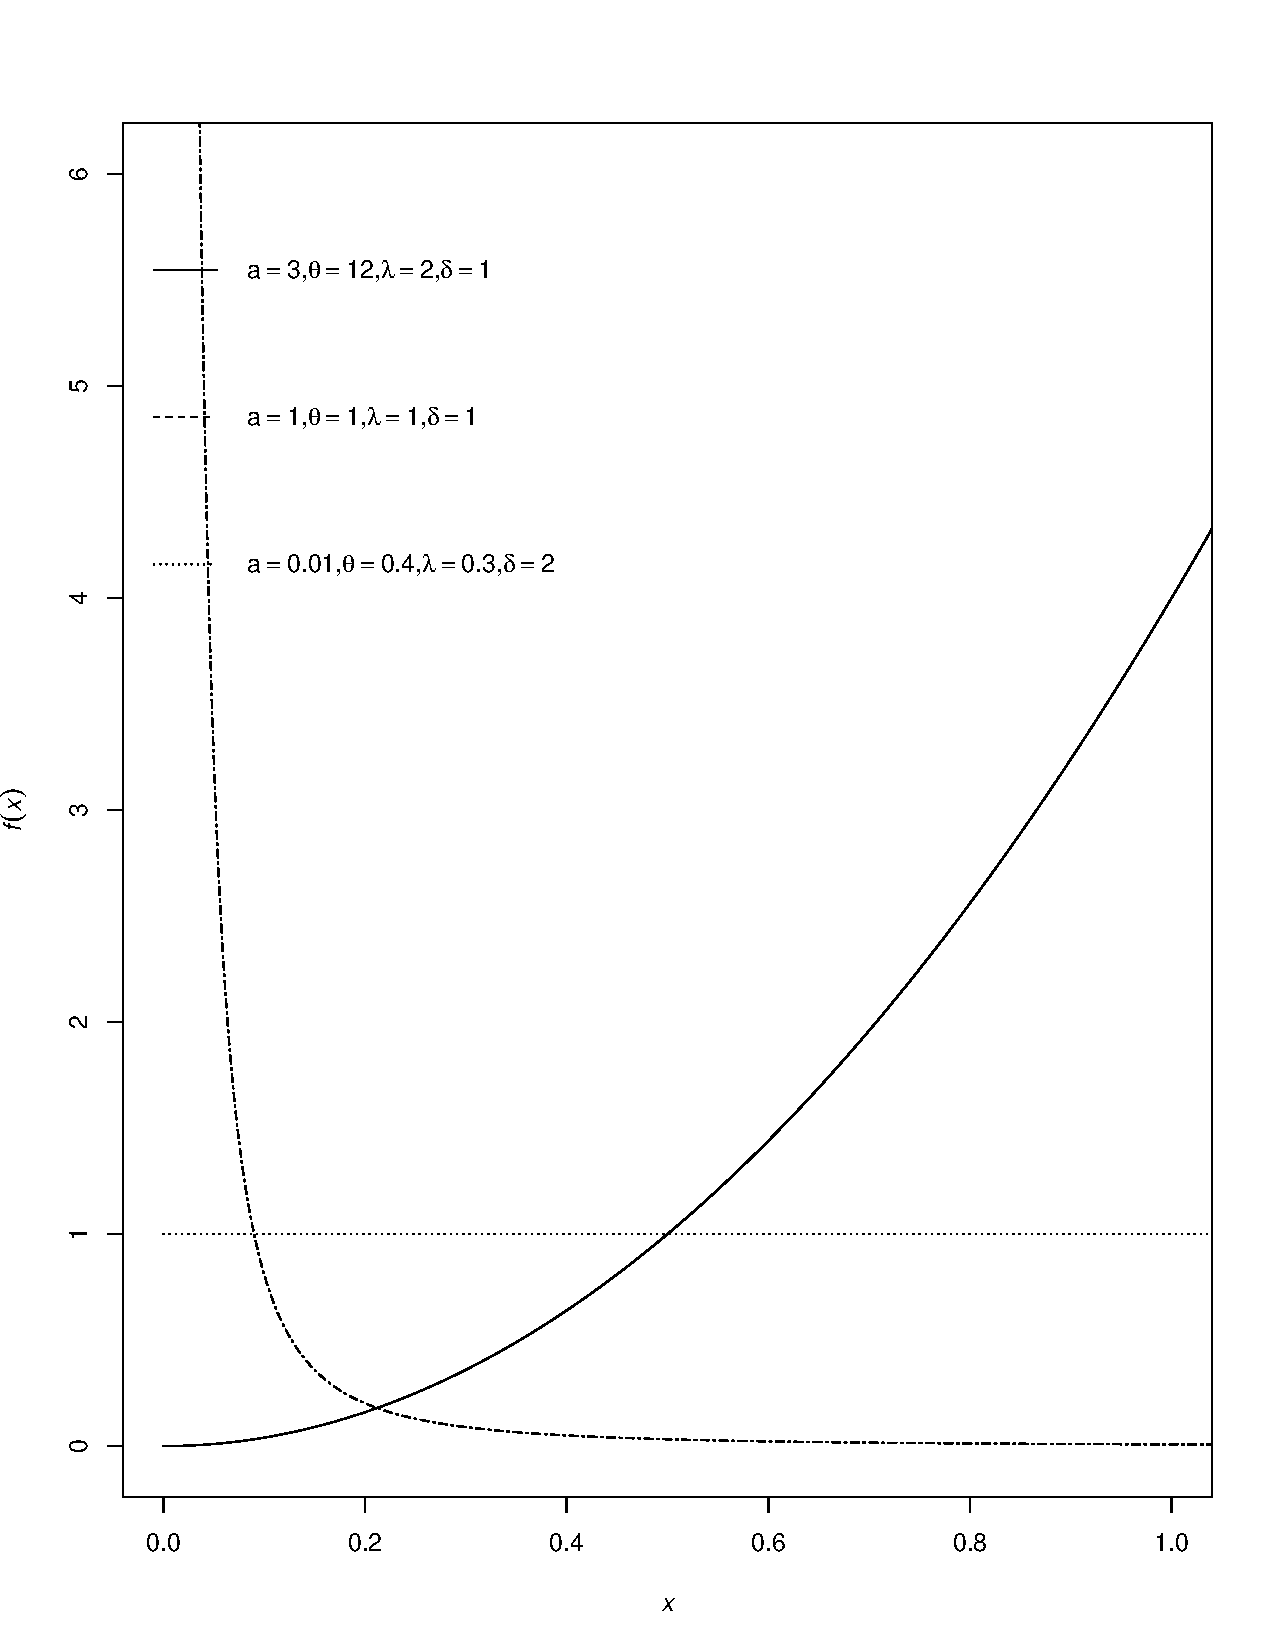
\includegraphics[scale=.3]{density.pdf}
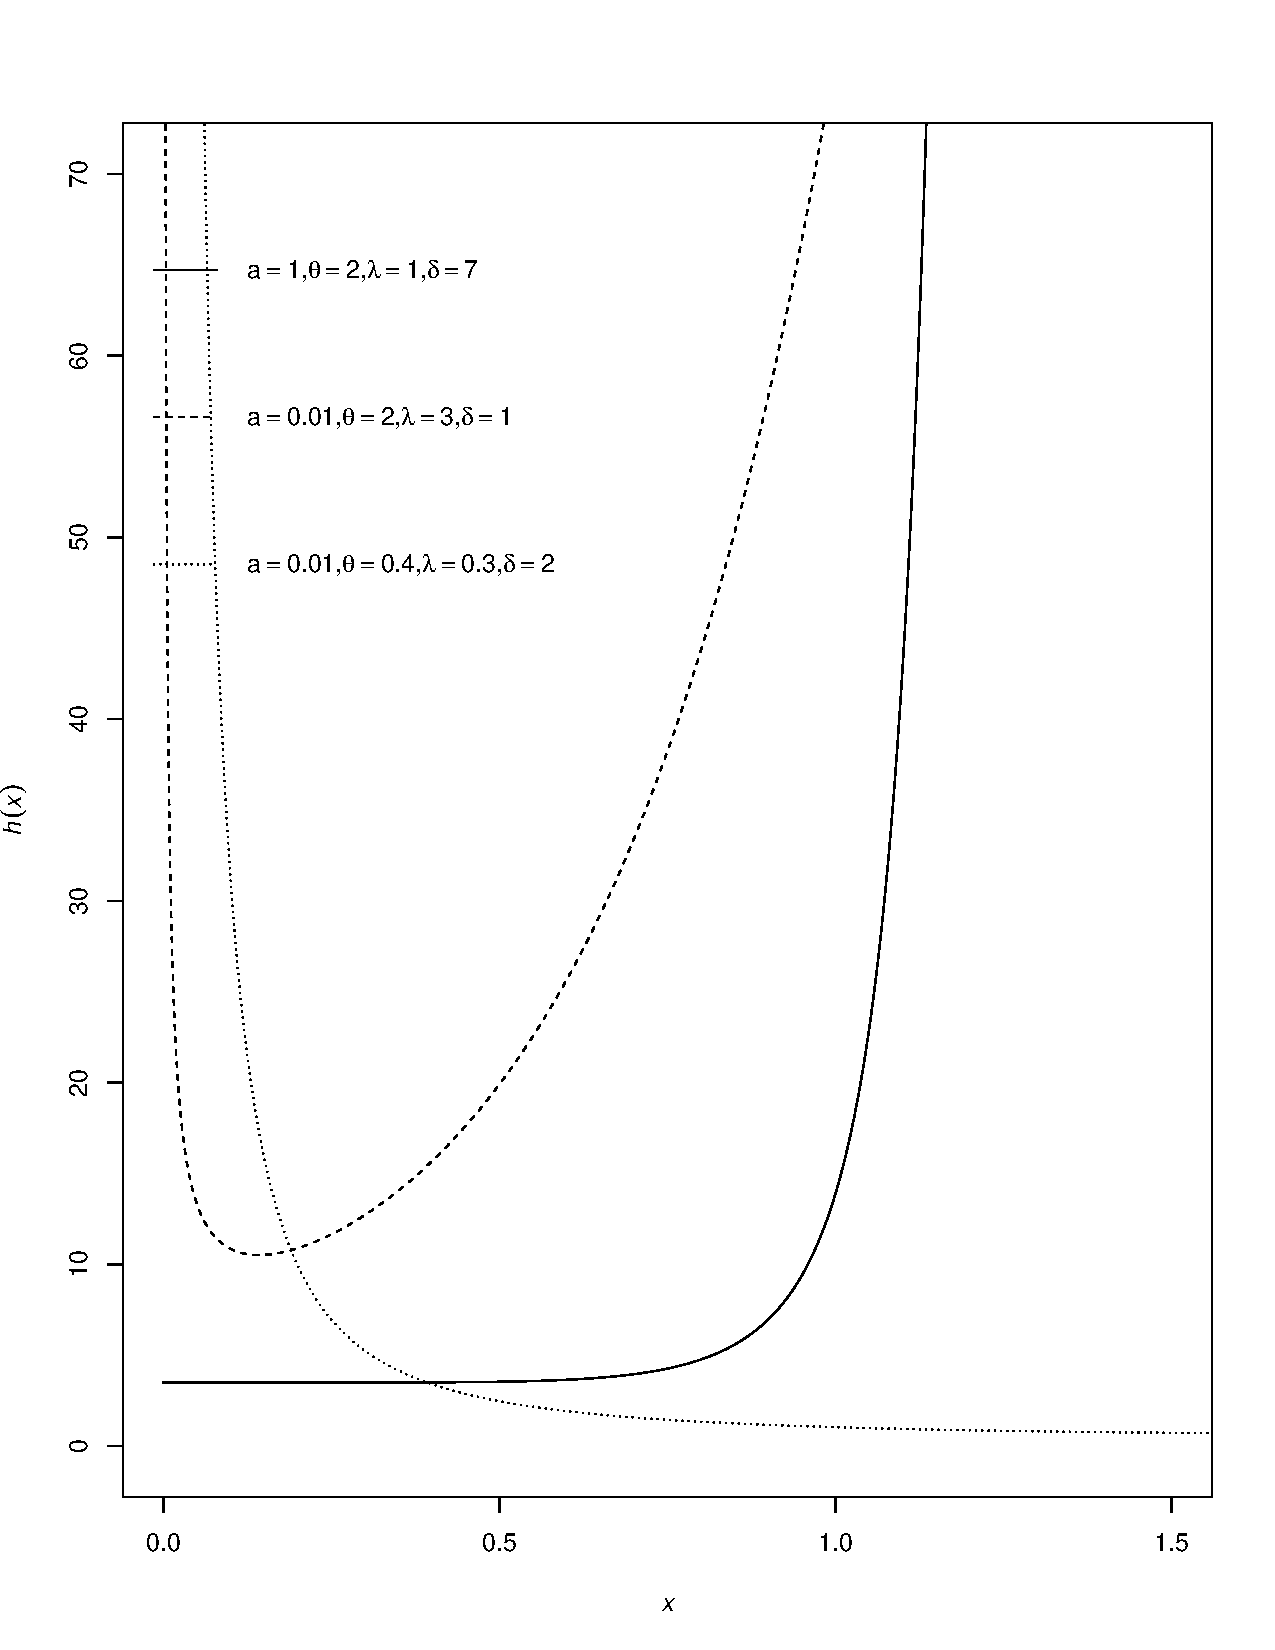
\includegraphics[scale=.3]{hazard.pdf}\\
\vspace{-0.5cm}
\caption{(a) Curves for the MO-$\Gamma$-W density; (b) Curves for the MO-$\Gamma$-W hazard;\label{formas}}
\end{center}
\end{figure}

\subsection{Quantile Function}\label{QuantFunc}

We can easily invert the cdf \eqref{CDF_MO-Gamma-G} to express the MOGa-G
quantile function (qf), say $x=Q_{X}(u)=G^{-1}(u)$, in terms of the baseline 
qf $Q_G(u)$. Let $u$ be a uniform $U(0,1)$ random variate. By using \eqref{CDF_MO-Gamma-G}
and letting $z=\gamma_{1}\left(a, -\log[1-G(x)]\right)$, we obtain $z=z(u)=\theta u/[1-(1-\theta)u]$. 
Then, the qf of $X$ has the form $x=Q_G\left(1-\rm{e}^{-v}\right)$, where $v=v(z)$ is a random variate generated
from a gamma distribution (with shape parameter $\alpha$ and unit scale parameter) corresponding to the quantile $z$. 
This scheme is useful because of the existence of fast generators for uniform and gamma 
random variables.

\section{Estimation}\label{estimation}

The  MO-$\Gamma$-G family mentioned previously can be  fitted to real data sets using the {\it AdequacyModel}
package for the {\sf R} statistical computing environment ({\tt https://www.r-project.org/}).
An important advantage of this packa\-ge is that it is not necessary to define
the log-likelihood function and that it computes the maximum likelihood estimates (MLE), their standard errors and the formal statistics
presented in the nest section. We only need to provide the PDF and CDF of the distribution to be fitted to a data set.
This {\it AdequacyModel} package uses the PSO (particle swarm optimization) method obtained by traditional global search approaches
such as the quasi-Newton BFGS, Nelder-Mead and simulated-annealing methods to maximized the log-likelihood function. This
method does not require initial values. More
details are available at {\tt https://rdrr.io/cran/AdequacyModel/}.

Here, we consider estimation of unknown parameters of the MO-$\Gamma$-$G$ distribution by the method of maximum likelihood. If $x$ is one observation from \ref{} and $\etn$ a q-vector parameter vector specifying $G(.)$, thus the log-likelihood function, say $\log L=\log L(a,\theta,\etn)$ is
\begin{align}\ell (\boldsymbol{\Theta})=&\,n\log (\theta)+n\log(\gamma)+n\, a\, \gamma \log(\lambda)+(a\gamma-1)\sum_{i=1}^n{\log(x_i)}-\lambda^\gamma\sum_{i=1}^n{\log(x_i)}-n\log[\Gamma(a)] \nonumber \\ & -2\sum_{i=1}^n{\log\{\theta+(1-\theta)\gamma_1[a,(\lambda\,x_i)^\gamma]\}}
\end{align}

\section{Simulation}\label{sec:simulation}

Due to the probable absence of maximum likelihood estimators - MLE in closed form for distributions belonging to the MO-$\Gamma $-G family, it is necessary to understand the precision of the estimates obtained numerically. For that, we chose to study the bias of the estimators of the MO-$\Gamma$-Dagum($\theta$, $a$, $\alpha$, $\beta$, $p$) distribution, in which $ G \sim \mathrm {Dagum} (\alpha, \beta, p) $, for different sample sizes, being (10, 20, 60, 100, 200, 400, 600, 1000, 2000, 5000, 10000, 20000, 30000 and 500000).

The simulations considered 10,000 Monte-Carlo - MC iterations for each of the sample sizes to which the numerical estimates were obtained by the BFGS method. Table \ref{tab:bias} shows that the BFGS method behaves well as the sample size grows. This is theoretically expected, however, in practice, difficulties can be faced in other families of distributions due to complications in the likelihood function.

All simulations can be reproduced using the code in Annex \ref {ap:simulation}. The MC simulations are parallelized and are able to use all threads available by a multicore processor, thus making them more computationally efficient and consequently requiring less time to complete. The simulations were performed on a computer with an Intel Core i5-8265U processor with 8 threads working at a maximum frequency of 3.90 GHz, requiring, on these hardware, a time of 14.36 hours to perform all simulations.

\begin{table}[H]
	\centering
	\caption{Mean bias of EMV obtained by the BFGS method in 10,000 Monte Carlo repetitions.} \label{tab:bias}
	\begin{tabular}{rrrrrrr}
		\hline
		$\bm n$ & $\bm B(\bm \hat{\bm \theta})$ & $\bm B(\bm \hat{\bm a})$ & $\bm B(\bm \hat{\bm \alpha})$ & $\bm B(\bm \hat{\bm \beta})$ & $\bm B(\bm \hat{\bm p})$ & \textbf{Time (mins)}\\ 
		\hline
		10 & 0.2376 & 2.1635 & 2.7557 & 1.6282 & 1.3057 & 1.1430\\ 
		20 & 0.4154 & 2.4639 & 1.5728 & 1.8082 & 0.7383 & 1.6248\\ 
		60 & 0.7214 & 2.2432 & 0.5667 & 1.8815 & 0.2872 & 3.3954\\ 
		100 & 0.6146 & 1.9579 & 0.3253 & 1.6148 & 0.2651 & 4.9628\\ 
		200 & 0.3838 & 1.3894 & 0.1827 & 1.1773 & 0.3701 & 8.1457\\ 
		400 & 0.2166 & 0.9635 & 0.1076 & 0.6181 & 0.3957 & 13.7370\\ 
		600 & 0.1269 & 0.7242 & 0.0772 & 0.3968 & 0.3637 & 17.9310\\ 
		1000 & 0.0553 & 0.4885 & 0.0521 & 0.2328 & 0.2636 & 22.8784 \\
		2000  &  0.0456 & 0.3087 &  0.0334 &  0.0990 & 0.1722 &  38.4593\\
		5000 & -0.0058 & 0.1307 & 0.0146 & 0.0117 & 0.0171 & 52.8098\\ 
		10000 & -0.0146 & 0.0842 & 0.0095 & 0.0095 & 0.0031 & 95.8380\\ 
		20000 & -0.0090 & 0.0330 & 0.0038 & 0.0005 & -0.0099 & 126.4260\\ 
		30000 & -0.0028 & 0.0183 & 0.0012 & -0.0036 & -0.0029 & 182.0760\\ 
		50000 & -0.0057 & 0.0124 & 0.0015 & 0.0016 & -0.0021 & 291.9300\\ 
		\hline
	\end{tabular}
\end{table}

\section{Applications}\label{applications}

In this section, we provide two applications in order to show the performance of our proposed family with another ones. To do this, we consider the Weibull distribution as baseline and for competitive distributions, we consider: beta-Weibull ($\beta$-W), proposed by Famoye {\it et al.} (2005); Kumaraswamy Weibull (KW-W), see Cordeiro and Nadarajah (2010); Marshall-Olkin Weibull (MO-W), studied by Ahmed {\it et al.} (2017); Marshall-Olkin Extented Weibull (MOE-W), see the family proposed by Cordeiro {\it et al.} (2019)
Exponentiated Weibull (exp-W), introduced by Mudholkar and Srivastava (1993); gamma Weibull (gamma-W), see Cordeiro {\it et al.} (2016) and exponentiated generalized Weibull (EG-W), see Oguntunde {\it et al.} (2015), with $a=1$.

The log-likelihood for the Marshall-Olkin Gamma Weibull (MO-$\Gamma$-W) and considering one observation is given by
\begin{align}
\ell (\boldsymbol{\Theta})=& \log (\theta)+\log (\gamma)+(a\,\gamma)\log (\lambda)+(a\,\gamma-1)\log(x)-(\gamma\, x)^\gamma-\log[\Gamma(a)]\nonumber \\ &-2\log\{\theta+(1-\theta)\gamma_1[a,(\lambda\,x)^\gamma]\}
\end{align}
where $\boldsymbol{\Theta}=(a,\theta,\lambda,\gamma)^T$. Besides that, the components of the score is given by

\begin{equation*}
U_{a}(\boldsymbol{\Theta})=\gamma  \log (\lambda )+\gamma  \log (x)-\psi ^{(0)}(a)-\frac{2\left\{(1-\theta ) A-(1-\theta ) \psi ^{(0)}(a) \gamma_1 \left[a,(x \lambda
   )^{\gamma }\right]\right\}}{\theta\,\Gamma(a)+(1-\theta)\gamma_1\left[a,(x \lambda
   )^{\gamma }\right]},
\end{equation*}

\begin{equation*}
U_{\theta}(\boldsymbol{\Theta})=\frac{1}{\theta}-\frac{2\left\{\Gamma(a)-\gamma_1\left[a,(\lambda\,x)^\gamma\right]\right\}}{\theta\,\Gamma(a)+(1-\theta)\gamma_1\left[a,(\lambda\,x)^\gamma\right]},
\end{equation*}

\begin{equation*}
U_{\lambda}(\boldsymbol{\Theta})=\frac{\gamma }{\lambda }\left[a-(\lambda\,x)^\gamma\right]+\frac{2 \gamma \,\lambda^{-1}(\lambda\,x)^{a\,\gamma} (1-\theta )\exp\{-(\lambda\,x)^\gamma\} }{\theta \,\Gamma(a)+(1-\theta )
   \gamma_1 \left[a,(x \lambda )^{\gamma }\right]}
\end{equation*}
and
\begin{equation*}		
U_{\gamma}\boldsymbol{\Theta}=\frac{1}{\gamma }+a \log (\lambda )+a \log (x)-(\lambda  x)^{\gamma } \log
   (\lambda  x)+\frac{2 (1-\theta )(\lambda 
   x)^{\gamma\,a } \log (\lambda  x)\exp\{-(\lambda  x)^{\gamma }\}  }{\theta \,\Gamma(a)+(1-\theta )
   \gamma_1 \left[a,(x \lambda )^{\gamma }\right]},
\end{equation*}
where
\begin{align*}
A=G_{2,3}^{3,0}\left[(x \lambda )^{\gamma }\Big{|}
\begin{array}{c}
 1,1 \\
 0,0,a \\
\end{array}
\right]+\log \left[(\lambda  x)^{\gamma }\right] \gamma_1 \left[a,(x \lambda )^{\gamma
   }\right].
\end{align*}
where $\psi^{(n)}(x)$ is the $n$-th derivative of the digamma function and
\begin{eqnarray*}
A=\psi^{(0)}(a) - \log\left[(\lambda x)^{\gamma}\right]-G^{3,0}_{2,3}\,\left((\lambda x)^{\gamma} \Big{|}	\stackrel{1,1}{0,0,a}\right),
\end{eqnarray*}
where $G^{m,n}_{p,q}\,\left(z \Big{|}	\stackrel{a_{1},\ldots,a_{p}}{b_{1},\ldots,b_{q}}\right)$ is the Meijer G function.%exp-W Mudholkar, G. S. and Srivastava, D. K. (1993). Exponentiatel Weibull family for analyzing bathtub failure-rate data. {\it IEEE Transactions on Reliability}, {\bf 42}, 299--302.

% kw-w Codeiro, G. M. and Nadarajah, S. (2010). The Kumaraswamy Weibull distribution with application to failure data. {\it Journal of the Franklin Institute}, {\bf 347}, 1399--1429.

%MO-W Ahmed, H. H., Bdair, O. M. and Ahsanullah, M. (2017). On Marshall-Olkin Extended Weibull distribution. {\it Journal of Statistical Theory and Methods}, {\bf 16}, 1--17.

%VER GAMMA WEIBULL (REFERENCIA MEU TRABALHO GAMMA EXTENDED WEIBULL CNO Journal of Statistical Distributions and Applications)

%EG-W Oguntunde, P. E., Odetunmibi, O. A. and Adejumo, A. O. (2015). On the Exponentiated Generalized Weibull Distribution: A Generalized of the Weibull Distribution. {\it Indian Journal of Science and Technology}, {\bf 8}, 1--7.

To provide the results, in this section we use the {\sf R} software. In order to adjust the data sets consider here, we use the {\it AdequacyModel} package mentioned in Section \ref{estimation}. The method used here was the SANN method, that is a variant of simulated annealing (Belisle, 1992). To compare our proposed model with the other ones mentioned above, we use the Anderson Darling (A$^{*}$) and Cramer Von Mises (W$^{*}$) statistics, given by the {\it goodness.fit} function.

For the first data set, we consider a modification of the ``FoodExpenditure'' from the {\it betareg} package in {\sf R} software, that refers  on proportion of income spent on food for a random sample of 38 households in a large US city, according to the package information. Here, we consider the household expenditures for food. The modification is
\begin{eqnarray*}
data = FoodExpenditure_{food} / \#(FoodExpenditure_{food}),
\end{eqnarray*}
where $FoodExpenditure_{food}$ is the random variable about the household expenditures for food and $\#(.)$ indicates the number of observations on the variable in question. The maximum likelihood estimators (MLE's) and their related standard errors (in parenthesis) are given in Table \ref{tab-ex1}. Besides that, the (W$^{*}$) and (A$^{*}$) statistics are described in this table too. The results indicate that the proposed model has better performance than the other ones.


\begin{table}[!htb]
\scriptsize
\center
\caption{  \small Application 1}
\label{tab-ex1}
\begin{tabular}{lcccccc}
\hline\noalign{\smallskip}
Model & $a$ & $\theta$ & $\lambda$ & $\gamma$ &  $W^*$ & $A^*$   \\
\hline \\
 & & & & &  \\
MO-$\Gamma$-W$(a,\theta,\lambda,\gamma)$    &  0.926134 & 1.379664 & 33.323073 & 25.398809 & 0.0339 &  0.2376 \\                            &    (0.02626926) & (0.22381086) & (0.28530971) & (0.08259864)  & & \\

 & & & & &  \\
$\beta-$W$(a,\theta,\lambda,\gamma)$ &   9.92882 &  0.1700880 & 9.759469 & 1.530541  & 0.043567 & 0.2594618\\
                                    &    (0.02908181) & (0.02049663) & ($<$0.0001) & ($<$0.0001)  && \\
                                                                                & & & & &  \\
KW-W$(a,\theta,\lambda,\gamma)$ &    0.04987575 & 99.99989793 &  1.07602954 & 23.40287099 & 1.330915 & 6.742609\\
                                       &    (0.008090352) & (16.225905058) &  (0.003156126) &  (0.014646102) && \\																						 & & & & &  \\
                                       MOE-W$(a,\theta,\lambda,\gamma)$  &  0.1366666 & 2.020436 & 62.72201 & 4.2956659  &0.03541554 & 0.2579222 \\
 & (0.1599182) & ($<$0.0001) &($<$0.0001) & (0.7365535)    &  & \\
                                                                              & & & & &  \\
EGW$(a,b,\lambda,\gamma)$    &  5.6189861421 &  6.1833138579 &  1.2870816760  & 1.3798562942  &  0.03715255 & 0.2518879 \\
& (0.0028147823) & (0.0009807091) & (0.1159810838) & (0.1480747352)    &  & \\
                                                           & & & & &  \\                                                           MO-W$(a,\lambda,\gamma)$  & 0.15920715  & - &  1.58609458  & 4.26713785  &  0.03456333   & 0.257339\\ 
&    (0.07170351) & (-) & (0.13353716) & (0.16650667)  &  & \\

 & & & & &  \\
exp-W$(a,\lambda,\gamma)$   &    6.1102948   & - &   4.4680469 &  1.3858740 &   0.03726684   & 0.2523749 \\
&   (0.4222173) & (-) & (0.3175876) & (0.1677722)   &  & \\

 & & & & &  \\
 gamma-W$(a,\lambda,\gamma)$    & 5.751546  & - &  10.0000 & 1.208773&  0.0879 & 0.6599  \\ 
&  (0.0015006)&  (-)&  (0.0001163185) &(0.00822782)    &  & \\

 & & & & &  \\





%GammaBS$(a,b,\alpha)$     &  1.2354 & 40.4438 &  0.1379 &       & 0.4931 &   2.7656 &  0.3725 & $1.765x10^{-12}$\\
                          %&  ( 0.0025)& ( 14.6913)& (0.0446) &      & &&  && \\
                                                     \hline
\end{tabular}
\end{table}



As a second application, we consider a data set that can be found in http://biostat.mc.vanderbilt.\\
edu/wiki/
Main/DataSets. This data was collected in a pilot study about hypertension in the Dominican Republic
in 1997. The observations are the systolic blood pressure of persons who came to medical clinics in
several villages, for a variety of complaints. The MLEs of the model parameters and standard errors
and the values of the statistics are listed in Table \ref{tab-ex2} for the previous models. Overall, by
comparing the measures of these formal goodness-of-fit statistics, we conclude that the proposed distribution
outperforms all distributions considered in Table \ref{tab-ex2}.

\begin{table}[htb!]
\scriptsize
\center
\caption{  \small Application 2}
\label{tab-ex2}
\begin{tabular}{lcccccc}
\hline\noalign{\smallskip}
Model & $a$ & $\theta$ & $\lambda$ & $\gamma$ &  $W^*$ & $A^*$   \\
\hline
 & & & & &  \\
MO-$\Gamma$-W$(a,\theta,\lambda,\gamma)$    &  9.629304 & 3.640779 & 6.260826 & 12.823429 &0.5093&  2.8076 \\
                                       &    (0.006217876) & (0.182495785) & (0.024446563) & (0.007965221)  && \\
                                       
 & & & & &  \\
 $\beta-$W$(a,\theta,\lambda,\gamma)$ &   31.08471 &  47.14636 &   0.01698383 &  2.054037 & 0.7540428 & 4.279418\\
&    (0.01279570) & ($<$0.0001) & (0.00014535) & ($<$0.0001)  && \\

 & & & & &  \\
KW-W$(a,\theta,\lambda,\gamma)$ &   7363.281 & 0.03925762 &  1.467640 &   0.6146940 & 0.5351 & 2.9617\\
                                       &    (0.04194304) & (0.0004194304)& ($<$0.0001)& ($<$0.0001) && \\

 & & & & &  \\
 MOE-W$(a,\theta,\lambda,\gamma)$  &  101.13471834 &  0.42386507  & 0.03095935 &  1.70240332  &1.14418 & 6.644617 \\
                            & (46.782882038) &  (0.100832102) &  (0.003644092) &  (0.168142275)   &  & \\
 
 & & & & &  \\
 EGW$(a,b,\lambda,\gamma)$    &  0.2351691 &  140.0000 &   0.4576370 &   0.7425738 &  0.8925 & 5.3338 \\
                            & (0.002540837) & (3.278565) & ($<$0.0001) & ($<$0.0001)   &  & \\
 
 & & & & &  \\
 MO-W$(a,\lambda,\gamma)$  & 173.2139  & - &  0.02125455 &  1.601970  &  1.476088   & 8.58705\\
                                       &    (0.00016394) & (-) & (0.000212794) & (0.0001398109)  &  & \\
                                       
 & & & & &  \\
 exp-W$(a,\lambda,\gamma)$   &    69.02916  & - &   0.02405120 & 1.345536 &   0.8899261   & 5.094141 \\
                          &   (0.08389090) & (-) & (0.0002249256) & ($<$0.0001)   &  & \\
                          
 & & & & &  \\
 gamma-W$(a,\lambda,\gamma)$    & 9.11229459   & - &  0.02617729 & 1.74641178 &    0.6227098 & 3.488268  \\ 
                             &  (0.96330688)&  (-)&  (0.00291875) & (0.08030313)     &  & \\
                             
 & & & & &  \\




%GammaBS$(a,b,\alpha)$     &  1.2354 & 40.4438 &  0.1379 &       & 0.4931 &   2.7656 &  0.3725 & $1.765x10^{-12}$\\
                          %&  ( 0.0025)& ( 14.6913)& (0.0446) &      & &&  && \\
                                                    \hline
\end{tabular}
\end{table}

\section{Mathematical properties}\label{properties}


In this section, we present some main mathematical properties for the MO-$\Gamma$-G family
based on a general linear representation for its density given in the next section.

\subsection{Linear Representation}


A linear representation for the PDF the new family defined previously
can be derived using the concept of exponentiated distributions.
For an arbitrary baseline CDF $G(x)$, the exponentiated-G (exp-G)
distribution with parameter $a>0$, has CDF and PDF in the forms
\begin{eqnarray*}
\Pi_a(x)=G(x)^a\qquad\text{and}\qquad\pi_a(x)=a\,g(x)\,G(x)^{a-1},
\end{eqnarray*}
respectively. The properties of the exponentiated distributions have been studied
by many authors in recent years, see Mudholkar and Srivastava (1995) for exponentiated
Weibull, Gupta {\it et al.} (1998) for exponentiated Pareto, Gupta and
Kundu (2001) for exponentiated exponential and Nadarajah and Gupta (2007)
for exponentiated gamma distribution. Tahir and Nadarajah (2015) cited almost
thirty exponentiated distributions in their Table 1.

A linear representation for the PDF of the MO-$\Gamma$-G family in terms of exp-G densities is important
to determine its mathematical properties from those of the exp-G distributions. They can follow from the papers
described below.

First, the MO-G density (\ref{densityMO}) admits the
linear combination  (Barreto-Souza \emph{et al.}, 2013)
\begin{equation*}
f_{\text{MO-G}}(x)
\,=\,
\sum^{\infty}_{i=0}\,w_i^{\text{MO-G}}\,\pi_{i+1}(x),
\label{EXP44}
\end{equation*}
where the coefficients are (for $i=0,1,\ldots$)
\[
w_i^{\text{MO-G}}=w_i^{\text{MO-G}}(\theta) =
\begin{cases}
\dfrac{(-1)^i\,\theta}{(i+1)} \sum\limits^{\infty}_{j=i}\dbinom{j}{i}(j+1) \bar{\theta}^j,& \quad \theta\in (0,1),\\
\theta^{-1} (1-\theta^{-1})^i,& \quad \theta>1,
\end{cases}
\]
and $\bar{\theta}=1-\theta$.


Second, the linear combination for the $\Gamma\text{-G}$ density (\ref{PDF_Ga}) was
derived by Castellares and Lemonte (2015) as
\begin{equation*}\label{EXP33}
f_{\Gamma\text{-G}}(x)\,=\,\sum_{i=0}^\infty w_i^{\Gamma\text{-G}}\,\,\pi_{a+i}(x),
\end{equation*}
where
$$w_i^{\Gamma\text{-G}}=w_i^{\Gamma\text{-G}}(a)=\frac{\varphi_{i}(a)}{(a+i)},$$
\begin{equation*}\label{coeficientes}
\varphi_0(a)=\frac{1}{\Gamma(a)},
\quad\,
\varphi_i(a)=\frac{(a-1)}{\Gamma(a)}\,\psi_{i-1}(i+a-2),\quad i\geq 1,
\end{equation*}
and
$\psi_{i-1}(\cdot)$ are the {\color{green}Stirling polynomials} defined by
\begin{align*}\label{polinomios_ward}
\begin{split}
\psi_{n-1}(x)&=\frac{(-1)^{n-1}}{(n+1)!}\Biggl[H^{n-1}_{n}-\frac{x+2}{n+2}H^{n-2}_{n}
+ \frac{(x+2)(x+3)}{(n+2)(n+3)}H^{n-3}_{n}- \cdots\\
&\qquad+ (-1)^{n-1}\frac{(x+2)(x+3)\cdots(x+n)}{(n+2)(n+3)\cdots(2n)}H^{0}_{n}\Biggr],
\end{split}
\end{align*}
where $H^{m}_{n}$ are positive integers given recursively by
$H^{m}_{n+1}=(2n+1-m)H^{m}_{n} + (n-m+1)H^{m-1}_{n}$, with
$H^0_0=1$, $H^{0}_{n+1}=1\times 3\times 5\times\cdots\times(2n+1)$, $H^{n}_{n+1}=1$.










\section{Conclusions}\label{conclusions}

Falta escrever ...


\appendix

\section{Simulation code}\label{ap:simulation}

The code below was used to perform the simulations whose results are found in Table \ref{tab:bias} of Section \ref{sec:simulation}. The code was developed using the programming language R and is available to be reused in other simulations or even to check the results presented in this paper.

\lstinputlisting[language=R, caption={Monte-Carlo simulations for different sample sizes.}, numbers=left,
stepnumber=1,
showspaces=false,
tabsize=4,  
basicstyle=\scriptsize,
backgroundcolor=\color{lbcolor},
showstringspaces=false]{new_code_dagum.R}


\section*{References}

\begin{description}

\item
A. Alzaatreh, F. Famoye, C. Lee:
A new method for generating families of continuous distributions.
Metron {\bf 71}(1) 63-79 (2013).

\item
W. Barreto-Souza, A.J. Lemonte, G.M. Cordeiro:
General results for the Marshall and Olkin's family of distributions.
Anais da Academia Brasileira de Ci\^{e}ncias {\bf 85}(1) 3-21 (2013).

\item
Z.W. Birnbaum, S.C. Saunders:
A new family of life distributions.
Journal of Applied Probability {\bf 6}(2) 319-327 (1969).

\item
F. Castellares, A.J. Lemonte:
A new generalized Weibull distribution gene\-rated by gamma random variables.
Journal of the Egyptian Mathematical Society {\bf 23}(2) 382-390 (2015).

\item
G.M. Cordeiro, M. de Castro:
A new family of generalized distributions.
Journal of Statistical Computation and Simulation {\bf 81}(7) 883-898 (2011).

\item
N. Eugene, C. Lee, F. Famoye:
Beta-normal distribution and its applications.
Communications in Statistics -- Theory and Methods {\bf 31}(4) 497-512 (2002).

\item
R.C. Gupta, R.D. Gupta, P.L. Gupta:
Modeling failure time data by Lehmann alternatives.
Communications in Statistics -- Theory and Methods {\bf 27}(4) 887-904 (1998).

\item
R.D. Gupta, D. Kundu:
Exponentiated exponential family: an alternative to gamma and Weibull distributions.
Biometrical Journal {\bf 43}(1) 117-130 (2001).

%\item
%P. Kumaraswamy:
%Generalized probability density-function for double-bounded
%random-processes. Journal of Hydrology {\bf 46}(1-2) 79-88 (1980).

\item
A.J. Lemonte, G.M. Cordeiro, G. Moreno-Arenas:
A new useful three-parameter extension of the exponential distribution.
Statistics {\bf 50}(2) 312-337 (2016).

\item
A.W. Marshall, I. Olkin:
A new method for adding a parameter to a family of distributions with
application to the exponential and Weibull families.
Biometrika {\bf 84}(3) 641-652 (1997).

\item
G.S. Mudholkar, D.K. Srivastava:
The exponentiated Weibull family: a reanalysis of the bus-motor-failure data.
Technometrics {\bf 37}(4) 436-445 (1995).

\item
S. Nadarajah, G.M. Cordeiro, E.M.M. Ortega:
Some general results for the beta-modified Weibull distribution.
Journal of Statistical Computation and Simulation {\bf 81}(10) 1211-1232 (2011).

\item
S. Nadarajah, G.M. Cordeiro, E.M.M. Ortega:
General results for the Kumaraswamy G distribution.
Journal of Statistical Computation and Simulation {\bf 87}(7) 951-979 (2012).

\item
S. Nadarajah, A.K. Gupta:
The exponentiated gamma distribution with application to drought data.
Calcutta Statistical Association Bulletin {\bf 59}(1-2) 29-54 (2007).

\item
S. Nadarajah, F. Haghighi:
An extension of the exponential distribution.
Statistics {\bf 45}(6) 543-558 (2011).

\item
S. Nadarajah, S. Kotz:
The exponentiated-type distributions.
Acta Applicandae Mathematicae {\bf 92}(2) 97-111 (2006).

\item
M.D. Nichols, W.J. Padgett:
A Bootstrap control chart for Weibull percentiles.
Quality and Reliability Engineering International {\bf 22}(2) 141-151 (2006).

\item
F. Proschan:
Theoretical explanation of observed decreasing failure rate.
Technometrics {\bf 5}(3) 375-383 (1963).

\item
M.M. Risti\'{c}, N. Balakrishnan:
The gamma-exponentiated exponential distribution.
Journal of Statistical Computation and Simulation {\bf 82}(8) 1191-1206 (2012).

\item
E.W. Stacy: A Generalization of the Gamma Distribution. Annals of Mathematical Statistics {\bf 33}(3) 1187-1192 (1962).

\item
M.H. Tahir, S. Nadarajah:
Parameter induction in continuous univariate distributions: Well-established G families.
Anais da Academia Brasileira de Ci\^{e}ncias {\bf 87}(2) 539-568 (2015).

\item
K. Zografos, N. Balakrishnan:
On families of beta-and generalized gamma-generated distribution and
associate inference.  Statistical Methodology {\bf 6}(4) 344-362 (2009).

\end{description}




\end{document}
